\documentclass[11pt,a4paper]{article}

% ── Packages ──
\usepackage[utf8]{inputenc}
\usepackage[T1]{fontenc}
\usepackage[margin=1in]{geometry}
\usepackage{amsmath,amssymb,mathtools}
\usepackage{bm}
\usepackage{xcolor}
\usepackage{hyperref}
\usepackage{listings}
\usepackage{booktabs}
\usepackage{enumitem}
\usepackage{tcolorbox}
\usepackage{longtable}
\usepackage{tikz}
\usetikzlibrary{arrows.meta,positioning,fit,calc}
\usepackage{fancyvrb}

\hypersetup{colorlinks=true,linkcolor=blue!70!black,citecolor=green!50!black,urlcolor=blue!60!black}

% ── Code style ──
\lstset{
  language=Python,
  basicstyle=\ttfamily\small,
  keywordstyle=\color{blue!70!black}\bfseries,
  commentstyle=\color{green!50!black}\itshape,
  stringstyle=\color{red!60!black},
  showstringspaces=false,
  breaklines=true,
  frame=single,
  backgroundcolor=\color{gray!5},
  numbers=left,
  numberstyle=\tiny\color{gray},
  xleftmargin=2em,
  framexleftmargin=1.5em
}

% ── Custom boxes ──
\newtcolorbox{filecard}[1]{colback=blue!3,colframe=blue!50!black,title={\small\texttt{#1}}}
\newtcolorbox{funccard}[1]{colback=green!3,colframe=green!60!black,title={\small\texttt{#1}}}
\newtcolorbox{outputguide}[1]{colback=orange!3,colframe=orange!50!black,title={\small Output Interpretation: #1}}
\newtcolorbox{warningbox}{colback=red!3,colframe=red!50!black,title={\small Warning}}
\newtcolorbox{tipbox}{colback=teal!3,colframe=teal!50!black,title={\small Tip}}

% ── Macros ──
\newcommand{\R}{\mathbb{R}}
\newcommand{\E}{\mathbb{E}}
\newcommand{\tr}{\operatorname{tr}}
\newcommand{\Normal}{\mathcal{N}}
\newcommand{\HalfCauchy}{\mathrm{C}^{+}}
\newcommand{\Spp}{\mathcal{S}^{+}_p}
\newcommand{\bOmega}{\bm{\Omega}}
\newcommand{\bSigma}{\bm{\Sigma}}

\title{\textbf{Codebase Reference Guide}\\[0.3em]
\large Sparse Bayesian Precision Matrix Estimation\\[0.3em]
\normalsize 6.7830 Final Project --- Spring 2026}
\author{Nick Bernardini \and Federico V.\ Cortesi \and Arturo Favara\\
\textit{Massachusetts Institute of Technology}}
\date{\today}

\begin{document}
\maketitle
\tableofcontents
\clearpage

%======================================================================
\part{Architecture Overview}
%======================================================================

\section{Project Directory Structure}

\begin{Verbatim}[fontsize=\small,frame=single]
bayesian_spm/
├── _info/                    Planning documents (proposals, reading plan, this guide)
├── data/
│   ├── raw/                  CRSP downloads, Fama-French factors (.gitignored)
│   ├── processed/            Cleaned (T x p) return matrices (.npy)
│   └── synthetic/            Generated (Omega, Y) pairs for validation
├── src/
│   ├── __init__.py
│   ├── models/
│   │   ├── __init__.py
│   │   └── graphical_horseshoe.py    Core NumPyro model
│   ├── inference/
│   │   ├── __init__.py
│   │   ├── nuts_runner.py            NUTS wrapper and sample extraction
│   │   └── advi_runner.py            ADVI wrapper with multi-seed restarts
│   ├── benchmarks/
│   │   ├── __init__.py
│   │   └── frequentist.py            Glasso, Ledoit-Wolf, sample covariance
│   ├── evaluation/
│   │   ├── __init__.py
│   │   └── metrics.py                Loss functions and sparsity metrics
│   ├── portfolio/
│   │   ├── __init__.py
│   │   └── gmv.py                    GMV weights, backtest engine
│   └── utils/
│       ├── __init__.py
│       ├── matrix_utils.py           Synthetic Omega generators, assembly
│       └── plotting.py               Heatmaps, ELBO traces, comparisons
├── notebooks/                Exploratory Jupyter notebooks
├── results/                  Saved posteriors (.npy) and metric tables (.json)
├── figures/                  Publication-quality plots (.pdf, .png)
├── paper/                    LaTeX source for the final report
├── tests/
│   ├── __init__.py
│   └── test_synthetic.py     Pytest suite for matrix generators
├── scripts/
│   └── run_experiment.py     CLI entry point for full experiments
├── environment.yml           Conda environment specification
├── .gitignore
└── README.md
\end{Verbatim}


\section{Dependency Graph Between Modules}

The following diagram shows which modules call which.  An arrow $A \to B$ means ``$A$ imports from $B$''.

\begin{center}
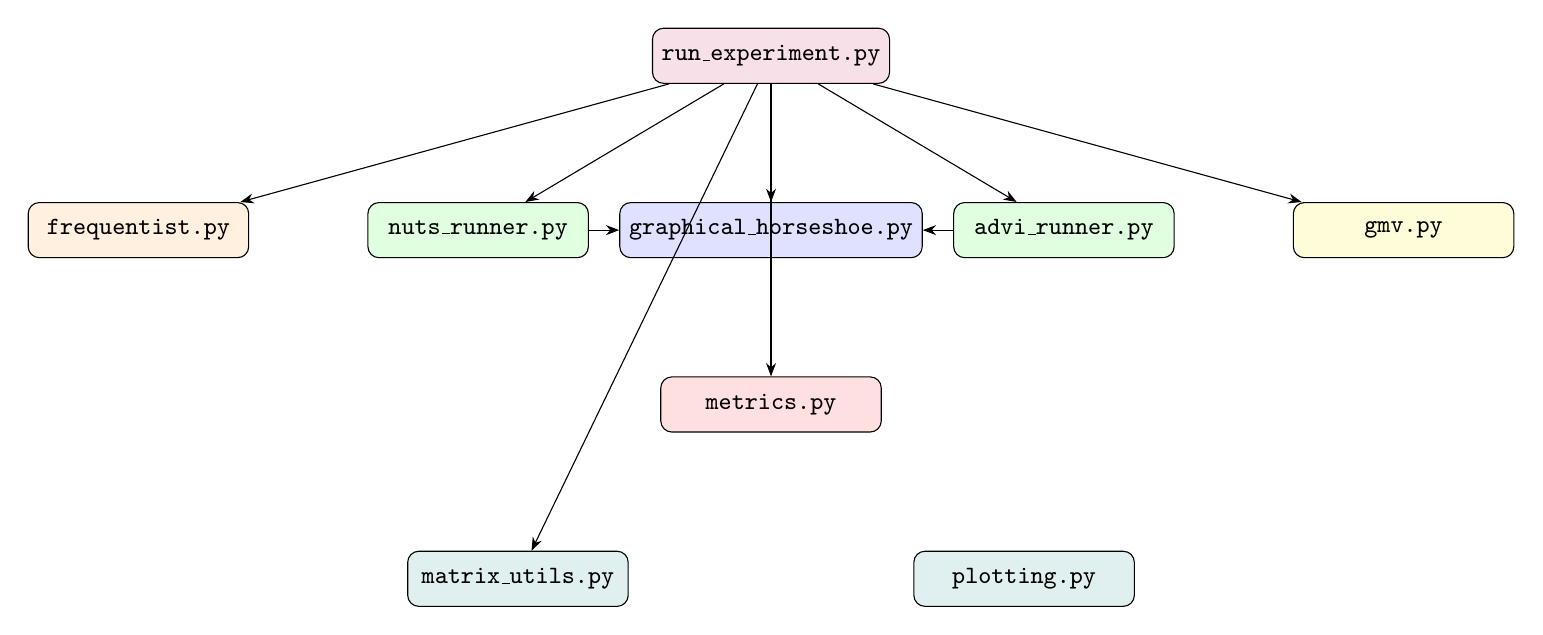
\begin{tikzpicture}[
  block/.style={rectangle, draw, rounded corners, minimum width=2.8cm, minimum height=0.7cm, font=\small\ttfamily, align=center},
  >=Stealth,
  node distance=1.4cm and 1.8cm
]

% Nodes
\node[block, fill=purple!12] (runner) {run\_experiment.py};
\node[block, fill=green!12, below left=1.5cm and 0.8cm of runner] (nuts) {nuts\_runner.py};
\node[block, fill=green!12, below right=1.5cm and 0.8cm of runner] (advi) {advi\_runner.py};
\node[block, fill=blue!12, below=1.5cm of runner] (model) {graphical\_horseshoe.py};
\node[block, fill=orange!12, left=1.5cm of nuts] (bench) {frequentist.py};
\node[block, fill=red!12, below=1.5cm of model] (metrics) {metrics.py};
\node[block, fill=teal!12, below left=1.5cm and 0.4cm of metrics] (matutils) {matrix\_utils.py};
\node[block, fill=teal!12, below right=1.5cm and 0.4cm of metrics] (plotting) {plotting.py};
\node[block, fill=yellow!15, right=1.5cm of advi] (gmv) {gmv.py};

% Edges
\draw[->] (runner) -- (nuts);
\draw[->] (runner) -- (advi);
\draw[->] (runner) -- (model);
\draw[->] (runner) -- (bench);
\draw[->] (runner) -- (metrics);
\draw[->] (runner) -- (matutils);
\draw[->] (nuts) -- (model);
\draw[->] (advi) -- (model);
\draw[->] (runner) -- (gmv);

\end{tikzpicture}
\end{center}

\noindent The key design principle is that every module depends only \emph{downward} in this graph:
\begin{itemize}[nosep]
  \item \texttt{run\_experiment.py} is the only orchestrator; it imports from all other modules.
  \item \texttt{nuts\_runner.py} and \texttt{advi\_runner.py} receive the model function as a parameter; they do not hard-import it.
  \item \texttt{metrics.py}, \texttt{matrix\_utils.py}, \texttt{plotting.py}, and \texttt{gmv.py} have no intra-project dependencies---they are pure utility modules.
\end{itemize}


\section{Data Flow Through the Pipeline}

A complete experiment proceeds in five stages:
\begin{enumerate}
  \item \textbf{Data generation} (\texttt{matrix\_utils.py}): Produce a ground-truth $\bOmega_0 \in \Spp$ and sample $\bm{Y} \in \R^{T \times p}$ from $\Normal(\bm{0}, \bOmega_0^{-1})$.
  \item \textbf{Inference} (\texttt{nuts\_runner.py} or \texttt{advi\_runner.py}): Feed $\bm{Y}$ and the \texttt{graphical\_horseshoe} model to the sampler/optimizer.  Produce posterior samples $\{\bOmega^{(s)}\}_{s=1}^S$.
  \item \textbf{Benchmarks} (\texttt{frequentist.py}): Run graphical lasso, Ledoit--Wolf, and sample covariance on the same $\bm{Y}$.
  \item \textbf{Evaluation} (\texttt{metrics.py}): Compare each $\hat\bOmega$ against $\bOmega_0$ via Stein's loss, Frobenius loss, spectral loss, and sparsity recovery.
  \item \textbf{Downstream} (\texttt{gmv.py}): Convert each $\hat\bOmega$ to GMV portfolio weights, and (optionally) run a rolling backtest.
\end{enumerate}

\noindent The CLI script \texttt{run\_experiment.py} executes stages 1--4 in a single invocation.  Stage 5 (portfolio) is currently invoked separately in notebooks or by extending the runner.


%======================================================================
\part{Module-by-Module Reference}
%======================================================================

%======================================================================
\section{\texttt{src/utils/matrix\_utils.py}}\label{sec:matutils}
%======================================================================

\begin{filecard}{src/utils/matrix\_utils.py}
\textbf{Purpose:} Synthetic precision matrix generation and low-level matrix assembly. This is the \emph{first} module to run in any experiment pipeline---it produces the ground-truth $\bOmega_0$ and the data $\bm{Y}$.
\\[0.3em]
\textbf{Dependencies:} \texttt{numpy}, \texttt{networkx}
\end{filecard}

\subsection{\texttt{assemble\_precision\_matrix(omega\_offdiag, omega\_diag, p)}}

\begin{funccard}{assemble\_precision\_matrix}
Takes a flat vector of $p(p-1)/2$ upper-triangular off-diagonal elements and a length-$p$ diagonal vector, and returns the full $(p \times p)$ symmetric matrix.
\end{funccard}

\paragraph{How it works.}
\begin{enumerate}[nosep]
  \item Allocates a $p \times p$ zero matrix.
  \item Fills the upper triangle (excluding diagonal) using \texttt{np.triu\_indices(p, k=1)}.
  \item Adds its own transpose to symmetrise: $\bOmega \leftarrow \bOmega + \bOmega^\top$.
  \item Sets the diagonal via \texttt{np.fill\_diagonal}.
\end{enumerate}

\paragraph{Index convention.} \texttt{np.triu\_indices(p, k=1)} returns indices in \textbf{row-major order}: $(0,1), (0,2), \ldots, (0,p{-}1), (1,2), \ldots, (p{-}2,p{-}1)$. This same ordering is used everywhere in the codebase (the NumPyro model, the NUTS extractor, the ADVI assembler). If you ever need to map a flat index $k$ back to a pair $(i,j)$, use:
\begin{lstlisting}
idx = np.triu_indices(p, k=1)
i, j = idx[0][k], idx[1][k]
\end{lstlisting}

\subsection{\texttt{\_graph\_to\_omega(G, p, signal\_range, rng)}}

\begin{funccard}{\_graph\_to\_omega \textnormal{(private helper)}}
Converts a NetworkX graph $G$ on $p$ nodes into a symmetric positive-definite precision matrix. This is the shared backend for all three graph generators.
\end{funccard}

\paragraph{Algorithm.}
\begin{enumerate}[nosep]
  \item Start with $\bOmega = \bm{I}_p$.
  \item For each edge $(i,j) \in G$, draw a sign $\in \{-1,+1\}$ uniformly and a magnitude from $\mathrm{Uniform}[\texttt{lo}, \texttt{hi}]$ where $(\texttt{lo}, \texttt{hi}) = \texttt{signal\_range}$.  Set $\omega_{ij} = \omega_{ji} = \text{sign} \times \text{magnitude}$.
  \item Record $(i,j)$ with $i < j$ in the edge set.
  \item Compute $\lambda_{\min}(\bOmega)$. If $\lambda_{\min} < 0.1$, shift the diagonal:
  \[
    \bOmega \leftarrow \bOmega + (0.1 - \lambda_{\min})\,\bm{I}_p.
  \]
  This guarantees $\bOmega \succ 0$ with a minimum eigenvalue of at least $0.1$.
\end{enumerate}

\begin{warningbox}
The diagonal shift changes the diagonal entries and therefore the marginal variances. It does \emph{not} change which off-diagonal entries are zero, so the sparsity pattern (conditional independence graph) is preserved. However, it does change the condition number $\kappa(\bOmega_0)$. Sparse graphs with many strong negative edges can produce very high condition numbers after the shift.
\end{warningbox}

\subsection{\texttt{sparse\_omega\_erdos\_renyi(p, sparsity, signal\_range, seed)}}

\begin{funccard}{sparse\_omega\_erdos\_renyi}
Generates $\bOmega_0$ with an Erd\H{o}s--R\'enyi random graph: each of the $\binom{p}{2}$ possible edges is included independently with probability \texttt{sparsity}.
\end{funccard}

\paragraph{Parameters.}
\begin{itemize}[nosep]
  \item \texttt{p}: dimension. Use $p=20$ for debugging, $p=50$ for main results, $p=100$ for scaling tests.
  \item \texttt{sparsity}: edge probability. At $\texttt{sparsity}=0.10$ with $p=50$, the expected number of edges is $\binom{50}{2} \times 0.10 = 122.5$.
  \item \texttt{signal\_range}: default $(0.3, 0.8)$. The absolute value of each nonzero $\omega_{ij}$ is drawn uniformly from this interval. Values below $0.2$ are difficult for any method to detect; values above $1.0$ may produce ill-conditioned matrices.
  \item \texttt{seed}: deterministic reproducibility via \texttt{np.random.default\_rng}.
\end{itemize}

\paragraph{Returns.}
\begin{itemize}[nosep]
  \item \texttt{Omega}: $(p \times p)$ positive-definite matrix.
  \item \texttt{edge\_set}: Python \texttt{set} of tuples $(i,j)$ with $i < j$. This is the ground-truth support, used later for computing TPR/FPR.
\end{itemize}

\subsection{\texttt{sparse\_omega\_band(p, bandwidth, signal\_range, seed)}}

\begin{funccard}{sparse\_omega\_band}
Generates a \textbf{banded} precision matrix: $\omega_{ij} \neq 0$ only if $|i - j| \le \texttt{bandwidth}$. This models local dependencies---e.g., stocks ordered by sector, where nearby stocks are more likely to be conditionally dependent.
\end{funccard}

\paragraph{Edge count.} For bandwidth $b$ and dimension $p$, the number of edges is exactly $\sum_{k=1}^{b}(p-k) = bp - b(b+1)/2$. For $p=50, b=2$: $98$ edges.

\subsection{\texttt{sparse\_omega\_block(p, n\_blocks, intra\_sparsity, signal\_range, seed)}}

\begin{funccard}{sparse\_omega\_block}
Generates a \textbf{block-diagonal} precision matrix: $p$ variables are split into \texttt{n\_blocks} groups, edges exist only within blocks, and within each block edges appear with probability \texttt{intra\_sparsity}. Models sector structure---stocks within the same industry share conditional dependencies, but are independent across sectors after conditioning.
\end{funccard}

\paragraph{Edge allocation.} The last block absorbs any remainder when $p$ is not divisible by \texttt{n\_blocks}. For $p=50$, $\texttt{n\_blocks}=5$: five blocks of 10 nodes each, with $\binom{10}{2} \times 0.3 = 13.5$ expected edges per block, $\approx 67.5$ edges total.

\subsection{\texttt{sample\_data\_from\_omega(Omega, T, seed)}}

\begin{funccard}{sample\_data\_from\_omega}
Given a positive-definite $\bOmega_0$, inverts it to obtain $\bSigma_0 = \bOmega_0^{-1}$ and draws $T$ i.i.d.\ samples $\bm{y}_k \sim \Normal(\bm{0}, \bSigma_0)$. Returns the $(T \times p)$ data matrix $\bm{Y}$.
\end{funccard}

\begin{outputguide}{Sanity checks after data generation}
After calling this function, verify:
\begin{enumerate}[nosep]
  \item $\bm{Y}$ has shape $(T, p)$ and is zero-mean (up to sampling noise): \texttt{np.abs(Y.mean(axis=0)).max()} should be $O(1/\sqrt{T})$.
  \item The sample covariance $\hat\bSigma = (T{-}1)^{-1}\bm{Y}^\top\bm{Y}$ has rank $\min(T{-}1, p)$.
  \item If $T > p$, $\hat\bSigma^{-1}$ exists and is ``reasonably close'' to $\bOmega_0$ (Frobenius error decreases with $T$).
\end{enumerate}
\end{outputguide}


%======================================================================
\section{\texttt{src/models/graphical\_horseshoe.py}}\label{sec:model}
%======================================================================

\begin{filecard}{src/models/graphical\_horseshoe.py}
\textbf{Purpose:} Defines the graphical horseshoe model as a NumPyro probabilistic program.  This single function is shared by both NUTS and ADVI---any difference in output is purely due to the inference method, not the model.
\\[0.3em]
\textbf{Dependencies:} \texttt{jax.numpy}, \texttt{numpyro}, \texttt{numpyro.distributions}
\end{filecard}

\subsection{The Generative Model}

The function \texttt{graphical\_horseshoe(Y, p, ncp, tau\_scale, diag\_prior)} encodes the following probabilistic model.  In the default non-centered parameterization (\texttt{ncp=True}):
\begin{align}
  \tau &\sim \HalfCauchy(0, \sigma_\tau), \label{eq:tau}\\
  \lambda_{ij} &\sim \HalfCauchy(0, 1), \quad \forall\; i < j, \label{eq:lambda}\\
  z_{ij} &\sim \Normal(0, 1), \quad \forall\; i < j, \label{eq:z}\\
  \omega_{ij} &= z_{ij} \cdot \lambda_{ij} \cdot \tau, \quad \forall\; i < j, \label{eq:omega_offdiag}\\
  \omega_{ii} &\sim \text{HalfNormal}(5), \quad \forall\; i, \label{eq:omega_diag}\\
  \bOmega &= \text{assemble}(\{\omega_{ij}\}_{i<j},\; \{\omega_{ii}\}_i), \quad \bOmega \in \Spp, \label{eq:assemble}\\
  \bm{y}_k &\sim \Normal(\bm{0}, \bOmega^{-1}), \quad k = 1,\ldots, T. \label{eq:lik}
\end{align}

\paragraph{Parameter count.} For dimension $p$:
\begin{itemize}[nosep]
  \item $1$ global shrinkage $\tau$
  \item $p(p{-}1)/2$ local shrinkage $\lambda_{ij}$
  \item $p(p{-}1)/2$ latent normals $z_{ij}$ (under NCP)
  \item $p$ diagonal elements $\omega_{ii}$
  \item \textbf{Total}: $D = 1 + p(p{-}1) + p = p^2 + 1$
\end{itemize}
For $p=50$: $D = 2{,}501$ parameters.  For $p=100$: $D = 10{,}001$.

\subsection{Non-Centered vs.\ Centered Parameterization}

\paragraph{Non-centered (default, \texttt{ncp=True}).} The sampler sees $z_{ij} \sim \Normal(0,1)$ and $\lambda_{ij} \sim \HalfCauchy(0,1)$ as separate latent variables, with $\omega_{ij}$ computed deterministically as the product $z_{ij} \cdot \lambda_{ij} \cdot \tau$. This breaks the strong posterior correlation between $\omega_{ij}$ and $\lambda_{ij}$ that arises in the centered form, which is critical for NUTS performance.

The non-centered parameterization is recommended when:
\begin{itemize}[nosep]
  \item The data is not highly informative about individual $\omega_{ij}$ (small $T$, weak signal).
  \item The horseshoe prior dominates the likelihood for many entries.
\end{itemize}

\paragraph{Centered (\texttt{ncp=False}).} The sampler directly samples $\omega_{ij} \sim \Normal(0, \lambda_{ij}^2 \tau^2)$. This is the ``textbook'' parameterization but creates a \emph{funnel geometry}: when $\lambda_{ij} \to 0$, the conditional variance of $\omega_{ij}$ shrinks to zero, trapping the sampler.  Use only if the non-centered version shows poor mixing (rare for this model).

\subsection{Diagonal Prior Options}

The diagonal elements $\omega_{ii}$ must be positive (they are marginal precisions). Three options:

\begin{center}
\begin{tabular}{@{}lll@{}}
\toprule
\texttt{diag\_prior} & Distribution & Properties \\
\midrule
\texttt{"halfnormal"} & $\text{HalfNormal}(5)$ & Mode at 0, mean $\approx 3.99$. Wide, weakly informative. \\
\texttt{"exponential"} & $\text{Exponential}(0.5)$ & Mode at 0, mean $= 2.0$. Heavier tail. \\
\texttt{"gamma"} & $\text{Gamma}(2, 0.5)$ & Mode at $2$, mean $= 4$. Pulls diagonal away from 0. \\
\bottomrule
\end{tabular}
\end{center}

\begin{tipbox}
For standardised return data (each stock divided by its sample standard deviation), the diagonal elements of $\bOmega$ represent inverse conditional variances, which are typically $O(1)$ to $O(10)$. The default \texttt{HalfNormal(5)} is appropriate. For raw returns with different volatilities, \texttt{Gamma(2, 0.5)} may be more suitable.
\end{tipbox}

\subsection{Assembly and Likelihood}

The function assembles $\bOmega$ using JAX's \texttt{.at[].set()} for differentiability:
\begin{lstlisting}
Omega = jnp.zeros((p, p))
idx_upper = jnp.triu_indices(p, k=1)
Omega = Omega.at[idx_upper].set(omega_offdiag)
Omega = Omega + Omega.T
Omega = Omega + jnp.diag(omega_diag)
\end{lstlisting}

The likelihood uses NumPyro's \texttt{MultivariateNormal} with \texttt{precision\_matrix=Omega}. Internally, NumPyro computes the Cholesky decomposition of $\bOmega$ to evaluate the log-density:
\[
  \log p(\bm{Y} \mid \bOmega) = \frac{T}{2}\log|\bOmega| - \frac{1}{2}\tr(\bm{S}\bOmega) - \frac{Tp}{2}\log(2\pi),
\]
where $\bm{S} = \sum_k \bm{y}_k\bm{y}_k^\top$. If the proposed $\bOmega$ is not positive definite, the Cholesky fails and NumPyro returns $-\infty$ log-density, causing the NUTS proposal to be rejected.

\begin{warningbox}
There is no explicit constraint enforcing $\bOmega \succ 0$ in the prior. Positive definiteness is enforced \emph{implicitly} by the likelihood: any non-PD proposal receives log-density $-\infty$. This means the sampler may waste proposals in early warmup. If you observe many divergent transitions, consider the Cholesky reparameterization described in the action plan.
\end{warningbox}


%======================================================================
\section{\texttt{src/inference/nuts\_runner.py}}\label{sec:nuts}
%======================================================================

\begin{filecard}{src/inference/nuts\_runner.py}
\textbf{Purpose:} Wraps NumPyro's NUTS sampler with sensible defaults, timing, and a helper to reconstruct full $\bOmega$ matrices from posterior samples.
\\[0.3em]
\textbf{Dependencies:} \texttt{jax}, \texttt{numpyro.infer.MCMC}, \texttt{numpyro.infer.NUTS}
\end{filecard}

\subsection{\texttt{run\_nuts(model, Y, p, ...)}}

\begin{funccard}{run\_nuts}
Initialises the NUTS kernel, creates a multi-chain \texttt{MCMC} object, runs warmup + sampling, prints the summary, and returns the fitted \texttt{MCMC} object.
\end{funccard}

\paragraph{Key parameters and their effects.}
\begin{center}
\begin{tabular}{@{}lp{9cm}@{}}
\toprule
Parameter & Effect \\
\midrule
\texttt{num\_warmup} (default 2000) & Number of adaptation steps per chain. During warmup, NUTS tunes the step size $\epsilon$ and mass matrix $\bm{M}$. Increase to 3000--5000 if you see poor $\hat{R}$ or low ESS. \\
\texttt{num\_samples} (default 5000) & Post-warmup samples per chain. Total samples = \texttt{num\_samples} $\times$ \texttt{num\_chains}. \\
\texttt{num\_chains} (default 4) & Independent Markov chains. Multiple chains are essential for computing $\hat{R}$. Minimum 2; standard is 4. \\
\texttt{target\_accept\_prob} (default 0.85) & Controls the adapted step size. Higher values $\to$ smaller $\epsilon$ $\to$ fewer divergences but slower exploration. Increase to 0.90--0.95 if divergences occur. \\
\texttt{max\_tree\_depth} (default 10) & Caps the binary tree depth in NUTS. Each additional level doubles the number of leapfrog steps. At depth 10, a single transition can take up to $2^{10} = 1024$ leapfrog steps. Increase to 12 if many transitions hit the depth limit (check \texttt{num\_steps} in the summary). \\
\bottomrule
\end{tabular}
\end{center}

\paragraph{What the function does internally.}
\begin{enumerate}[nosep]
  \item Converts $\bm{Y}$ to a JAX array.
  \item Creates a \texttt{NUTS} kernel with the given \texttt{target\_accept\_prob} and \texttt{max\_tree\_depth}.
  \item Creates an \texttt{MCMC} object wrapping that kernel, with \texttt{progress\_bar=True}.
  \item Runs \texttt{mcmc.run(rng\_key, Y=Y\_jnp, p=p)}.
  \item Prints the summary table and wall-clock time.
  \item Returns the \texttt{MCMC} object.
\end{enumerate}

\begin{outputguide}{NUTS summary table}
The printed summary contains one row per parameter (or parameter group). Key columns:
\begin{itemize}[nosep]
  \item \textbf{mean, std}: Posterior mean and standard deviation across all chains.
  \item \textbf{median}: Posterior median.
  \item \textbf{5.0\%, 95.0\%}: 90\% credible interval.
  \item \textbf{n\_eff}: Effective sample size (ESS). Should be $> 400$ for reliable posterior summaries. If $< 100$ for any parameter, the chain has not mixed.
  \item \textbf{r\_hat} ($\hat{R}$): Gelman--Rubin convergence diagnostic. Must be $< 1.01$ for all parameters. Values $> 1.1$ indicate the chains have not converged; do not trust the results.
\end{itemize}
Also check:
\begin{itemize}[nosep]
  \item \textbf{Number of divergences}: Printed at the top. Should be 0. If $> 0$, increase \texttt{target\_accept\_prob} or switch to the centered parameterization.
  \item \textbf{Wall-clock time}: Expect minutes for $p=20$, tens of minutes to hours for $p=50$, potentially infeasible for $p=100$.
\end{itemize}
\end{outputguide}

\subsection{\texttt{extract\_omega\_samples(mcmc, p)}}

\begin{funccard}{extract\_omega\_samples}
Takes a fitted \texttt{MCMC} object and reconstructs a 3D array of shape \texttt{(n\_samples, p, p)} containing the full symmetric precision matrix at each posterior draw.
\end{funccard}

\paragraph{How it handles both parameterizations.}
\begin{itemize}[nosep]
  \item If \texttt{ncp=True} was used: the MCMC samples contain \texttt{z}, \texttt{lambdas}, \texttt{tau}, and \texttt{omega\_offdiag} (a deterministic site). The function uses \texttt{omega\_offdiag} directly if available, otherwise recomputes it as $z \cdot \lambda \cdot \tau$.
  \item The function uses \texttt{jax.vmap} to vectorise the assembly over all $S$ samples, avoiding a Python loop.
\end{itemize}

\paragraph{Typical usage.}
\begin{lstlisting}
mcmc = run_nuts(graphical_horseshoe, Y, p=50)
Omega_samples = extract_omega_samples(mcmc, p=50)
Omega_mean = Omega_samples.mean(axis=0)    # posterior mean estimate
Omega_median = np.median(Omega_samples, axis=0)  # posterior median
\end{lstlisting}


%======================================================================
\section{\texttt{src/inference/advi\_runner.py}}\label{sec:advi}
%======================================================================

\begin{filecard}{src/inference/advi\_runner.py}
\textbf{Purpose:} Runs ADVI (Automatic Differentiation Variational Inference) via NumPyro's SVI interface, with multiple random restarts to handle initialisation sensitivity, and returns posterior samples from the best-performing guide.
\\[0.3em]
\textbf{Dependencies:} \texttt{jax}, \texttt{numpyro.infer.SVI}, \texttt{numpyro.infer.autoguide.*}, \texttt{numpyro.optim.Adam}
\end{filecard}

\subsection{Guide Types}

The \texttt{GUIDE\_MAP} dictionary maps string names to NumPyro autoguide classes:

\begin{center}
\begin{tabular}{@{}llp{6.5cm}@{}}
\toprule
\texttt{guide\_type} & NumPyro class & Description \\
\midrule
\texttt{"mean\_field"} & \texttt{AutoNormal} & Independent Gaussian in unconstrained space. $O(D)$ variational parameters (mean + log-scale per latent). Fastest but worst approximation. \\
\texttt{"full\_rank"} & \texttt{AutoMultivariateNormal} & Full-covariance Gaussian. $O(D^2)$ parameters (Cholesky factor). Best Gaussian approximation but may be infeasible for $p \ge 50$ ($D \approx 2500$, Cholesky has $\sim 3$M entries). \\
\texttt{"low\_rank"} & \texttt{AutoLowRankMVN} & Low-rank-plus-diagonal covariance: $\bm{L}\bm{L}^\top + \bm{D}$. $O(Dr)$ parameters for rank $r$. Good middle ground. \\
\texttt{"map"} & \texttt{AutoDelta} & Point mass at the MAP estimate. No uncertainty quantification. Use as a degenerate baseline. \\
\bottomrule
\end{tabular}
\end{center}

\subsection{\texttt{run\_advi(model, Y, p, ...)}}

\begin{funccard}{run\_advi}
Runs SVI with \texttt{Trace\_ELBO} loss for \texttt{num\_steps} iterations, repeated from \texttt{num\_seeds} different random initialisations. Keeps the run with the lowest final loss. Draws \texttt{num\_samples} from the best guide.
\end{funccard}

\paragraph{Multi-seed protocol.}
ADVI optimises a non-convex objective (the negative ELBO). Different initialisations can converge to different local optima. The function:
\begin{enumerate}[nosep]
  \item For each seed $s = 0, 1, \ldots, \texttt{num\_seeds}{-}1$: creates a fresh guide and SVI object with \texttt{PRNGKey(rng\_seed + s)}, runs \texttt{num\_steps} optimisation steps, records the final loss.
  \item Selects the seed with the \emph{lowest} final loss (= highest ELBO).
  \item Draws posterior samples from that guide via \texttt{numpyro.infer.Predictive}.
\end{enumerate}

\paragraph{Returns.} A dictionary with:
\begin{itemize}[nosep]
  \item \texttt{"samples"}: dict of JAX arrays, keyed by site name (\texttt{tau}, \texttt{lambdas}, \texttt{z}, \texttt{omega\_diag}, etc.). Shape \texttt{(num\_samples, ...)} for each site.
  \item \texttt{"losses"}: list of per-iteration loss values (negative ELBO) for the best seed. Plot with \texttt{plot\_elbo\_trace()}.
  \item \texttt{"guide\_params"}: optimised parameters of the best guide (can be saved/reloaded).
  \item \texttt{"best\_seed"}: index of the winning seed.
  \item \texttt{"all\_final\_losses"}: list of final losses across all seeds. Large spread $\Rightarrow$ high initialisation sensitivity.
  \item \texttt{"elapsed\_seconds"}: total wall-clock time across all seeds.
\end{itemize}

\begin{outputguide}{ADVI diagnostics}
\begin{enumerate}[nosep]
  \item \textbf{ELBO trace} (\texttt{losses}): should converge to a plateau. If still decreasing at the end, increase \texttt{num\_steps}. If oscillating wildly, reduce \texttt{learning\_rate}.
  \item \textbf{Spread of final losses} (\texttt{all\_final\_losses}): compute \texttt{np.std(all\_final\_losses)}. Large standard deviation (relative to the mean) indicates the ELBO landscape has many local optima---the horseshoe posterior is multimodal and mean-field cannot capture this.
  \item \textbf{ELBO gap}: if you have the MCMC marginal likelihood estimate $\log p(\bm{Y})$, then $\log p(\bm{Y}) - \text{ELBO}_{\text{final}} \approx \text{KL}(q \| p)$. A large gap means the variational approximation is poor.
  \item \textbf{PSIS diagnostic}: use ArviZ to compute Pareto $\hat{k}$ values by importance-sampling VI samples toward the MCMC posterior. $\hat{k} > 0.7$ indicates serious approximation failure.
\end{enumerate}
\end{outputguide}

\begin{warningbox}
The ADVI runner prints intermediate ELBO values every 10,000 steps. If the loss is \texttt{nan} or \texttt{inf}, the optimisation has diverged. This can happen with the horseshoe model because the half-Cauchy's heavy tail causes gradient explosions. Remedies:
\begin{itemize}[nosep]
  \item Reduce \texttt{learning\_rate} to $0.005$ or $0.001$.
  \item Use gradient clipping (requires replacing \texttt{Adam} with \texttt{ClippedAdam}).
  \item Switch to \texttt{"low\_rank"} guide (fewer parameters, more stable).
\end{itemize}
\end{warningbox}


%======================================================================
\section{\texttt{src/benchmarks/frequentist.py}}\label{sec:benchmarks}
%======================================================================

\begin{filecard}{src/benchmarks/frequentist.py}
\textbf{Purpose:} Provides three frequentist estimators of $\bSigma$ and $\bOmega$ as baselines.
\\[0.3em]
\textbf{Dependencies:} \texttt{numpy}, \texttt{sklearn.covariance}
\end{filecard}

\subsection{\texttt{run\_sample\_cov(Y)}}

\begin{funccard}{run\_sample\_cov}
Computes the unbiased sample covariance $\hat\bSigma = (T{-}1)^{-1}\bm{Y}^\top\bm{Y}$ via \texttt{np.cov(Y, rowvar=False, bias=False)}.
Returns $\hat\bOmega = \hat\bSigma^{-1}$ if $T > p$ and $\hat\bSigma$ is invertible; otherwise returns \texttt{None}.
\end{funccard}

\begin{outputguide}{When \texttt{Omega\_hat} is \texttt{None}}
This happens when $T \le p$ (the sample covariance is rank-deficient) or when $\hat\bSigma$ is numerically singular. This is expected behaviour---it's precisely the regime where regularisation is needed. In the experiment runner, a \texttt{None} result means this method is excluded from the metrics comparison.
\end{outputguide}

\subsection{\texttt{run\_ledoit\_wolf(Y)}}

\begin{funccard}{run\_ledoit\_wolf}
Computes the Ledoit--Wolf (2004) linear shrinkage estimator:
\[
  \hat\bSigma_{\text{LW}} = \hat\alpha\,\mu\bm{I} + (1 - \hat\alpha)\,\hat\bSigma,
\]
where $\hat\alpha \in [0,1]$ is the analytically optimal shrinkage intensity and $\mu = \tr(\hat\bSigma)/p$.
\end{funccard}

\paragraph{Returns.}
\begin{itemize}[nosep]
  \item \texttt{Sigma\_hat}: the shrunk covariance $(p \times p)$.
  \item \texttt{Omega\_hat}: its inverse $(p \times p)$. Always exists because the shrinkage target $\mu\bm{I}$ ensures positive definiteness.
  \item \texttt{shrinkage\_intensity}: the estimated $\hat\alpha$. Values near 1 mean the sample covariance is very noisy (high $p/T$); values near 0 mean the sample covariance is trustworthy (low $p/T$).
\end{itemize}

\subsection{\texttt{run\_glasso(Y, alphas, cv)}}

\begin{funccard}{run\_glasso}
Fits the graphical lasso (Friedman, Hastie, Tibshirani, 2008) with cross-validation:
\[
  \hat\bOmega_{\text{GL}} = \arg\max_{\bOmega \succ 0}\;\left\{\log|\bOmega| - \tr(\hat\bSigma\,\bOmega) - \rho\sum_{i \neq j}|\omega_{ij}|\right\},
\]
where $\rho$ is selected by 5-fold CV (or using the grid \texttt{alphas}).
\end{funccard}

\paragraph{Key notes.}
\begin{itemize}[nosep]
  \item \texttt{assume\_centered=True} because the data is already demeaned.
  \item \texttt{alpha\_selected}: the CV-optimal regularisation strength. Larger $\rho$ $\to$ sparser $\hat\bOmega$.
  \item The graphical lasso produces exactly-zero off-diagonal entries, making it directly comparable to the horseshoe's shrinkage profile.
\end{itemize}


%======================================================================
\section{\texttt{src/evaluation/metrics.py}}\label{sec:metrics}
%======================================================================

\begin{filecard}{src/evaluation/metrics.py}
\textbf{Purpose:} Computes all evaluation metrics comparing an estimated $\hat\bOmega$ against a ground-truth $\bOmega_0$. Used only with synthetic data (where $\bOmega_0$ is known).
\\[0.3em]
\textbf{Dependencies:} \texttt{numpy} only.
\end{filecard}

\subsection{Loss Functions}

\subsubsection{\texttt{steins\_loss(Omega\_hat, Omega\_true)}}

\begin{funccard}{steins\_loss}
Stein's loss (also known as the \emph{entropy loss} or \emph{KL divergence loss}):
\[
  L_S = \tr(\hat\bOmega^{-1}\bOmega_0) - \log|\hat\bOmega^{-1}\bOmega_0| - p.
\]
Equivalently, $L_S = \text{KL}(\Normal(0, \hat\bOmega^{-1}) \| \Normal(0, \bOmega_0^{-1}))$ up to a constant factor.
\end{funccard}

\paragraph{Implementation.} Computes $\bm{M} = \hat\bOmega^{-1}\bOmega_0$ via \texttt{np.linalg.solve} (avoids explicit inversion), then $L_S = \tr(\bm{M}) - \log|\bm{M}| - p$ where $\log|\bm{M}|$ is computed via \texttt{np.linalg.slogdet}.

\begin{outputguide}{Interpreting Stein's loss}
\begin{itemize}[nosep]
  \item $L_S = 0$ if and only if $\hat\bOmega = \bOmega_0$ (perfect recovery).
  \item $L_S > 0$ always (it is a Bregman divergence).
  \item \textbf{Not symmetric}: $L_S(\hat\bOmega, \bOmega_0) \neq L_S(\bOmega_0, \hat\bOmega)$.
  \item Stein's loss penalises \emph{eigenvalue distortion}: if $\hat\bOmega$ has the right eigenvectors but wrong eigenvalues, the loss is $\sum_i (\hat\lambda_i/\lambda_i^{(0)} - \log(\hat\lambda_i/\lambda_i^{(0)}) - 1)$.
  \item \textbf{Scale}: for $p=50$, a Stein's loss of $\sim 5$--$10$ is typical for a good estimator at $p/T \approx 0.5$. At $p/T \approx 1$, the sample covariance may have $L_S > 100$.
\end{itemize}
\end{outputguide}

\subsubsection{\texttt{frobenius\_loss(Omega\_hat, Omega\_true)}}

\begin{funccard}{frobenius\_loss}
$L_F = \|\hat\bOmega - \bOmega_0\|_F^2 = \sum_{i,j}(\hat\omega_{ij} - \omega_{ij}^{(0)})^2.$
\end{funccard}

\paragraph{Interpretation.} Simple elementwise comparison.  Sensitive to large errors in any single entry.  For $p = 50$, there are $p^2 = 2{,}500$ entries, so even small per-element errors accumulate.  Useful to compare across methods on the same problem, but the raw number is hard to interpret in isolation; consider the \emph{relative} Frobenius loss $L_F / \|\bOmega_0\|_F^2$.

\subsubsection{\texttt{spectral\_loss(Omega\_hat, Omega\_true)}}

\begin{funccard}{spectral\_loss}
$L_2 = \|\hat\bOmega - \bOmega_0\|_2 = \lambda_{\max}(\hat\bOmega - \bOmega_0)$ (largest singular value of the difference).
\end{funccard}

\paragraph{Interpretation.} Measures the worst-case distortion in any direction.  More stringent than Frobenius: a single badly-estimated eigenvalue makes $L_2$ large even if all other eigenvalues are correct.

\subsection{Sparsity Recovery Metrics}

\subsubsection{\texttt{sparsity\_metrics(Omega\_hat, Omega\_true, threshold)}}

\begin{funccard}{sparsity\_metrics}
Computes a full suite of binary classification metrics treating edge detection as a binary problem: for each off-diagonal pair $(i,j)$ with $i < j$, the ``true label'' is whether $|\omega_{ij}^{(0)}| > \texttt{threshold}$, and the ``predicted label'' is whether $|\hat\omega_{ij}| > \texttt{threshold}$.
\end{funccard}

\paragraph{Returned metrics.}
\begin{center}
\begin{tabular}{@{}lp{8cm}@{}}
\toprule
Key & Formula and interpretation \\
\midrule
\texttt{"tpr"} & True positive rate (sensitivity/recall): $\text{TP}/(\text{TP}+\text{FN})$. Fraction of true edges recovered. \\
\texttt{"fpr"} & False positive rate: $\text{FP}/(\text{FP}+\text{TN})$. Fraction of true zeros incorrectly declared as edges. \\
\texttt{"precision"} & $\text{TP}/(\text{TP}+\text{FP})$. Of the declared edges, what fraction are correct. \\
\texttt{"recall"} & Same as TPR. \\
\texttt{"f1"} & $2 \cdot \text{precision} \cdot \text{recall} / (\text{precision} + \text{recall})$. Harmonic mean; single-number summary. \\
\texttt{"mcc"} & Matthews correlation coefficient: $(\text{TP}\cdot\text{TN} - \text{FP}\cdot\text{FN}) / \sqrt{(\text{TP}+\text{FP})(\text{TP}+\text{FN})(\text{TN}+\text{FP})(\text{TN}+\text{FN})}$. Best single metric for imbalanced problems (our graphs are sparse $\Rightarrow$ mostly negatives). \\
\bottomrule
\end{tabular}
\end{center}

\begin{tipbox}
For Bayesian estimators, the posterior mean $\hat\bOmega = \bar\bOmega$ will generally have \emph{no} entries exactly equal to zero (the horseshoe shrinks toward zero but never reaches it). The \texttt{threshold} parameter determines the cutoff. A natural Bayesian alternative is to declare edge $(i,j)$ present if the $95\%$ credible interval for $\omega_{ij}$ excludes zero---this requires posterior samples, not just the mean.
\end{tipbox}


%======================================================================
\section{\texttt{src/portfolio/gmv.py}}\label{sec:gmv}
%======================================================================

\begin{filecard}{src/portfolio/gmv.py}
\textbf{Purpose:} Converts precision matrix estimates into portfolio weights and runs a rolling-window out-of-sample backtest.
\\[0.3em]
\textbf{Dependencies:} \texttt{numpy}, \texttt{pandas}
\end{filecard}

\subsection{\texttt{gmv\_weights(Omega)}}

\begin{funccard}{gmv\_weights}
Computes the global minimum variance portfolio weights:
\[
  \bm{w}^* = \frac{\bOmega\,\bm{1}}{\bm{1}^\top\bOmega\,\bm{1}}.
\]
This is the closed-form solution to $\min_{\bm{w}} \bm{w}^\top\bSigma\bm{w}$ subject to $\bm{w}^\top\bm{1} = 1$. The key insight is that it depends on $\bOmega = \bSigma^{-1}$ directly, so we never need to invert back to $\bSigma$.
\end{funccard}

\paragraph{Properties of the output.}
\begin{itemize}[nosep]
  \item Weights sum to 1 by construction.
  \item Weights can be \textbf{negative} (short positions). The horseshoe's shrinkage reduces the magnitude of off-diagonal elements, which tends to produce more concentrated, less extreme weights compared to the sample covariance inverse.
  \item For a posterior distribution over $\bOmega$, you can call \texttt{gmv\_weights} on each sample to get a \emph{posterior distribution over weights}.
\end{itemize}

\subsection{\texttt{portfolio\_variance(w, Sigma)}}

\begin{funccard}{portfolio\_variance}
Computes $\sigma_p^2 = \bm{w}^\top\bSigma\bm{w}$. Used for in-sample portfolio risk evaluation.
\end{funccard}

\subsection{\texttt{rolling\_backtest(returns\_df, estimation\_fn, window\_size, rebalance\_freq)}}

\begin{funccard}{rolling\_backtest}
Implements a rolling-window out-of-sample portfolio backtest. At each rebalancing date, estimates $\hat\bOmega$ from the trailing \texttt{window\_size} days of returns, computes GMV weights, and holds the portfolio until the next rebalancing date.
\end{funccard}

\paragraph{Protocol.}
\begin{enumerate}[nosep]
  \item Identify rebalancing dates by resampling the DataFrame's date index at frequency \texttt{rebalance\_freq} (\texttt{"M"} = monthly, \texttt{"Q"} = quarterly, \texttt{"W"} = weekly).
  \item At each rebalancing date $t$:
  \begin{enumerate}[nosep]
    \item Extract the in-sample window $\bm{Y}_{[t - T, t)}$.
    \item Call \texttt{estimation\_fn(Y\_window)} to obtain $\hat\bOmega$.
    \item Compute $\bm{w}_t = \texttt{gmv\_weights}(\hat\bOmega)$.
    \item Compute out-of-sample daily returns: $r_t^{\text{pf}} = \bm{w}_t^\top \bm{r}_t$ for each day until the next rebalancing date.
  \end{enumerate}
  \item Aggregate across all rebalancing periods.
\end{enumerate}

\paragraph{Returned metrics.}
\begin{center}
\begin{tabular}{@{}lp{8.5cm}@{}}
\toprule
Key & Description \\
\midrule
\texttt{"portfolio\_returns"} & Numpy array of daily out-of-sample portfolio returns. \\
\texttt{"weights\_history"} & Dict mapping rebalancing dates to weight vectors. \\
\texttt{"volatility\_oos"} & Annualised out-of-sample volatility: $\hat\sigma \times \sqrt{252}$. \textbf{Primary comparison metric.} Lower is better. \\
\texttt{"sharpe\_ratio"} & Annualised Sharpe ratio: $\sqrt{252} \cdot \bar{r} / \hat\sigma$. \\
\texttt{"max\_drawdown"} & Largest peak-to-trough decline in cumulative returns. Always negative. \\
\texttt{"turnover"} & Average $\ell_1$ distance between consecutive weight vectors: $\bar{\text{TO}} = \frac{1}{N}\sum_t \|\bm{w}_t - \bm{w}_{t-1}\|_1$. High turnover implies high transaction costs. \\
\bottomrule
\end{tabular}
\end{center}

\begin{outputguide}{Which estimator ``wins''?}
The primary downstream metric is \texttt{volatility\_oos}. The estimator that produces the lowest annualised out-of-sample volatility is the most effective for portfolio construction. However, also check:
\begin{itemize}[nosep]
  \item \textbf{Turnover}: If NUTS produces slightly lower volatility but 10$\times$ higher turnover, the advantage vanishes after transaction costs.
  \item \textbf{Sharpe ratio}: Accounts for both return and risk, but is noisier than volatility in short samples.
  \item \textbf{Weight stability}: Plot weight vectors over time. Erratic weight swings indicate estimation instability.
\end{itemize}
\end{outputguide}


%======================================================================
\section{\texttt{src/utils/plotting.py}}\label{sec:plotting}
%======================================================================

\begin{filecard}{src/utils/plotting.py}
\textbf{Purpose:} Publication-quality visualisation functions. All functions accept an optional \texttt{ax} parameter for embedding into multi-panel figures; if \texttt{None}, they create their own figure.
\\[0.3em]
\textbf{Dependencies:} \texttt{numpy}, \texttt{matplotlib}, \texttt{seaborn}
\end{filecard}

\subsection{\texttt{plot\_precision\_heatmap(Omega, title, ax, vmax)}}

Renders a diverging heatmap (blue = negative, white = zero, red = positive) of $\bOmega$ using \texttt{seaborn.heatmap}. Off-diagonal entries are coloured symmetrically around zero; the diagonal is typically larger and may dominate the colour scale, so \texttt{vmax} is auto-set from the off-diagonal maximum.

\paragraph{Use case.} Compare the true $\bOmega_0$ (left panel) against estimates from NUTS, ADVI, and glasso (right panels) in a single figure.

\subsection{\texttt{plot\_shrinkage\_profile(kappa\_nuts, kappa\_advi, ax)}}

Plots side-by-side histograms of the posterior shrinkage coefficient $\hat\kappa_{ij} = \E[1/(1 + \lambda_{ij}^2\tau^2) \mid \bm{Y}]$ for NUTS and ADVI.

\paragraph{What to look for.} The horseshoe's defining property is \emph{bimodal} shrinkage: most $\hat\kappa_{ij}$ should cluster near 0 (no shrinkage $\Rightarrow$ edge present) or near 1 (full shrinkage $\Rightarrow$ edge absent), with few values in between.
\begin{itemize}[nosep]
  \item \textbf{NUTS}: should show a clear bimodal distribution if the model is working correctly.
  \item \textbf{ADVI (mean-field)}: expected to collapse the bimodality into a \emph{unimodal} distribution peaked near the mean. This is the paper's main hypothesis.
\end{itemize}

\subsection{\texttt{plot\_eigenvalue\_comparison(eigenvalues\_dict, true\_eigenvalues, ax)}}

Overlays sorted eigenvalue spectra for multiple estimators. The true spectrum (solid black) is plotted alongside each method (dashed colours).

\paragraph{What to look for.}
\begin{itemize}[nosep]
  \item The sample covariance eigenvalues will be spread too wide (Mar\v{c}enko--Pastur effect).
  \item Ledoit--Wolf linearly shrinks eigenvalues toward the grand mean.
  \item The graphical lasso and horseshoe should better preserve the shape of the true spectrum.
\end{itemize}

\subsection{\texttt{plot\_elbo\_trace(losses, title, ax)}}

Plots the ELBO ($= -\texttt{loss}$) over optimisation iterations. Overlays a raw trace (grey, thin) and a moving-average smoothed trace (blue, thick) with window size $\min(500, N/10)$.

\paragraph{What to look for.}
\begin{itemize}[nosep]
  \item \textbf{Convergence}: the smoothed curve should plateau.
  \item \textbf{Oscillation}: large oscillations even late in training suggest the learning rate is too high.
  \item \textbf{Sudden drops/spikes}: may indicate numerical instability in the guide or likelihood.
\end{itemize}

\subsection{\texttt{plot\_posterior\_comparison(omega\_nuts, omega\_advi, omega\_true, entry\_labels, ax)}}

For selected $\omega_{ij}$ entries, plots overlaid histograms of NUTS posterior (blue) and ADVI posterior (coral), with the true value as a vertical dashed line.

\paragraph{What to look for.}
\begin{itemize}[nosep]
  \item \textbf{Bias}: Is the ADVI posterior centred at the wrong location?
  \item \textbf{Variance}: Is the ADVI posterior too narrow (overconfident)? Too wide?
  \item \textbf{Shape}: For entries near zero, the NUTS posterior may be sharply peaked at zero with a heavy tail; the ADVI posterior will be Gaussian (in unconstrained space).
\end{itemize}


%======================================================================
\section{\texttt{scripts/run\_experiment.py}}\label{sec:runner}
%======================================================================

\begin{filecard}{scripts/run\_experiment.py}
\textbf{Purpose:} Command-line entry point that orchestrates a complete experiment: data generation (or loading), inference, evaluation, and result serialisation.
\\[0.3em]
\textbf{Dependencies:} All \texttt{src/} modules.
\end{filecard}

\subsection{Command-Line Interface}

\paragraph{Basic usage.}
\begin{lstlisting}[language=bash]
# Run NUTS on synthetic data (p=50, T=250, Erdos-Renyi, 10% sparsity)
python scripts/run_experiment.py --synthetic --p 50 --T 250 --method nuts

# Run ADVI mean-field with 3 random restarts
python scripts/run_experiment.py --synthetic --p 50 --T 250 --method advi \
  --guide mean_field --num-seeds 3

# Run ALL methods (NUTS + ADVI + glasso + LW + sample cov)
python scripts/run_experiment.py --synthetic --p 50 --T 250 --method all

# Use band graph instead of Erdos-Renyi
python scripts/run_experiment.py --synthetic --p 50 --T 120 --graph band

# Run on real (pre-processed) data
python scripts/run_experiment.py --p 50 --T 250 --method nuts
\end{lstlisting}

\paragraph{Full argument reference.}
\begin{center}
\small
\begin{longtable}{@{}llp{5.5cm}@{}}
\toprule
\textbf{Argument} & \textbf{Default} & \textbf{Description} \\
\midrule
\texttt{--p} & 50 & Dimension (number of stocks / variables). \\
\texttt{--T} & 250 & Sample size (number of trading days / observations). \\
\texttt{--method} & \texttt{nuts} & Inference method. One of: \texttt{nuts}, \texttt{advi}, \texttt{glasso}, \texttt{ledoit\_wolf}, \texttt{sample\_cov}, \texttt{all}. \\
\texttt{--guide} & \texttt{mean\_field} & ADVI guide type (only used if method is \texttt{advi}). \\
\texttt{--synthetic} & \texttt{False} & Use synthetic data with known ground truth. \\
\texttt{--sparsity} & 0.10 & Edge probability (Erd\H{o}s--R\'enyi) or intra-block sparsity. \\
\texttt{--graph} & \texttt{erdos\_renyi} & Graph structure: \texttt{erdos\_renyi}, \texttt{band}, or \texttt{block}. \\
\texttt{--seed} & 42 & Master random seed. \\
\texttt{--output-dir} & \texttt{results/} & Directory for saved outputs. \\
\midrule
\multicolumn{3}{@{}l}{\textbf{NUTS-specific}} \\
\texttt{--num-warmup} & 2000 & Warmup steps per chain. \\
\texttt{--num-samples} & 5000 & Posterior samples per chain. \\
\texttt{--num-chains} & 4 & Number of chains. \\
\texttt{--target-accept} & 0.85 & NUTS target acceptance probability. \\
\midrule
\multicolumn{3}{@{}l}{\textbf{ADVI-specific}} \\
\texttt{--num-steps} & 50000 & SVI optimisation steps. \\
\texttt{--learning-rate} & 0.01 & Adam learning rate. \\
\texttt{--num-seeds} & 5 & Number of random restarts. \\
\bottomrule
\end{longtable}
\end{center}

\subsection{Internal Flow}

\begin{enumerate}
  \item \textbf{Data}: If \texttt{--synthetic}, calls \texttt{generate\_synthetic\_data()} which dispatches to the appropriate graph generator in \texttt{matrix\_utils.py} and then samples data. Otherwise, loads a preprocessed \texttt{.npy} file from \texttt{data/processed/returns\_p\{p\}.npy}.
  \item \textbf{Method dispatch}: For \texttt{nuts} or \texttt{advi}, calls \texttt{run\_bayesian\_method()} which imports the model and the appropriate runner. For frequentist methods, calls \texttt{run\_frequentist\_method()}.
  \item \textbf{Evaluation}: If a ground-truth $\bOmega_0$ exists (synthetic data only), calls \texttt{evaluate()} which computes all metrics from \texttt{metrics.py}.
  \item \textbf{Serialisation}: Saves $\hat\bOmega$ as \texttt{results/omega\_\{tag\}.npy} and the metrics summary as \texttt{results/metrics\_p\{p\}\_T\{T\}.json}.
\end{enumerate}

\subsection{Output Files}

\paragraph{Per-method:} \texttt{results/omega\_\{method\}\_p\{p\}\_T\{T\}\_\{graph\}\_s\{seed\}.npy} --- a $(p \times p)$ numpy array of the point estimate (posterior mean for Bayesian, regularised estimate for frequentist).

\paragraph{Summary:} \texttt{results/metrics\_p\{p\}\_T\{T\}.json} --- a JSON array of dictionaries, one per method, each containing:
\begin{lstlisting}[language={}]
{
  "method": "nuts",
  "steins_loss": 3.142,
  "frobenius_loss": 12.71,
  "spectral_loss": 1.05,
  "tpr": 0.87,
  "fpr": 0.03,
  "mcc": 0.82,
  "f1": 0.85,
  "precision": 0.83,
  "recall": 0.87,
  "elapsed_seconds": 347.2
}
\end{lstlisting}

\begin{outputguide}{Console output}
For each method, the runner prints:
\begin{itemize}[nosep]
  \item A separator bar and method name.
  \item NUTS: the full summary table (see Section~\ref{sec:nuts}).
  \item ADVI: intermediate ELBO values every 10k steps, plus final summary.
  \item All methods: the five key metrics (Stein's, Frobenius, spectral, F1, MCC) and wall-clock time.
\end{itemize}
\end{outputguide}


%======================================================================
\section{\texttt{tests/test\_synthetic.py}}\label{sec:tests}
%======================================================================

\begin{filecard}{tests/test\_synthetic.py}
\textbf{Purpose:} Pytest suite validating the synthetic data generators. These are \emph{property-based} tests: they verify structural invariants (positive definiteness, symmetry, sparsity range) rather than comparing against hardcoded values.
\\[0.3em]
\textbf{Run with:} \texttt{pytest tests/test\_synthetic.py -v}
\end{filecard}

\subsection{Test Inventory}

\begin{center}
\begin{tabular}{@{}lp{6cm}l@{}}
\toprule
\textbf{Test} & \textbf{What it checks} & \textbf{Parametrised over} \\
\midrule
\texttt{test\_erdos\_renyi\_is\_pd} & All eigenvalues of $\bOmega$ are $> 0$ & $p \in \{10, 20, 50\}$ \\
\texttt{test\_erdos\_renyi\_is\_symmetric} & $\bOmega = \bOmega^\top$ (elementwise) & $p \in \{10, 20, 50\}$ \\
\texttt{test\_band\_is\_pd} & Band matrix is positive definite & $p \in \{10, 20, 50\}$ \\
\texttt{test\_block\_is\_pd} & Block matrix is positive definite & $p \in \{20, 50\}$ \\
\texttt{test\_erdos\_renyi\_sparsity} & Observed edge fraction is in $(0.01, 0.30)$ when $s=0.10$ & $p = 50$ \\
\bottomrule
\end{tabular}
\end{center}

\begin{tipbox}
These tests run in seconds and should be executed after any modification to \texttt{matrix\_utils.py}.  If you add new graph generators (e.g., star, scale-free), add corresponding \texttt{test\_*\_is\_pd} and \texttt{test\_*\_is\_symmetric} tests.
\end{tipbox}


%======================================================================
\part{Interpreting Experiment Results}
%======================================================================

\section{Recommended Experiment Progression}

\begin{enumerate}
  \item \textbf{Smoke test} ($p=10$, $T=500$, ER, $s=0.10$): Run NUTS with 500 warmup, 1000 samples, 2 chains. Should complete in under a minute. Verify $\hat{R} < 1.01$, no divergences, posterior mean is visually close to $\bOmega_0$.
  \item \textbf{Core configuration} ($p=50$, $T=250$, ER, $s=0.10$): Run all five methods. This is the main result for the paper. NUTS may take 30--120 minutes; ADVI 5--15 minutes; frequentist methods seconds.
  \item \textbf{Scaling in $T$}: Fix $p=50$, vary $T \in \{75, 120, 250, 500\}$. Plot each metric as a function of $p/T$. The key finding is where the Bayesian methods start to diverge from frequentist methods.
  \item \textbf{Scaling in $p$}: Try $p=100$, $T=250$. NUTS may be infeasible; if so, report this as a finding and use ADVI + frequentist only.
  \item \textbf{Graph structure sensitivity}: Run the core configuration with \texttt{--graph band} and \texttt{--graph block}.
\end{enumerate}

\section{Key Comparisons for the Paper}

\subsection{NUTS vs.\ ADVI (Inference Quality)}

This is the paper's central comparison. Focus on:
\begin{enumerate}[nosep]
  \item \textbf{Point estimates}: Stein's loss, Frobenius loss for NUTS posterior mean vs.\ ADVI posterior mean.
  \item \textbf{Shrinkage profiles}: Use \texttt{plot\_shrinkage\_profile} to show bimodality (NUTS) vs.\ unimodality (ADVI).
  \item \textbf{Sparsity recovery}: F1 and MCC. Does ADVI recover the same edges as NUTS?
  \item \textbf{Posterior calibration}: For each $\omega_{ij}$, compute the 95\% credible interval from NUTS and ADVI. Check coverage against the true value. ADVI is expected to have lower coverage (overconfident).
  \item \textbf{Computation time}: NUTS wall-clock vs.\ ADVI wall-clock. Plot the quality--speed tradeoff.
\end{enumerate}

\subsection{Bayesian vs.\ Frequentist (Regularisation Quality)}

\begin{enumerate}[nosep]
  \item \textbf{Stein's loss comparison}: At which $p/T$ ratio does the graphical horseshoe beat the graphical lasso? At which ratio does Ledoit--Wolf suffice?
  \item \textbf{Eigenvalue spectrum}: Use \texttt{plot\_eigenvalue\_comparison} to show which estimator best preserves the true spectrum.
  \item \textbf{Portfolio performance}: Which estimator yields the lowest out-of-sample volatility?
\end{enumerate}

\section{Common Failure Modes and Debugging}

\begin{center}
\begin{longtable}{@{}p{4cm}p{4cm}p{5cm}@{}}
\toprule
\textbf{Symptom} & \textbf{Likely cause} & \textbf{Fix} \\
\midrule
NUTS divergences & Funnel geometry from half-Cauchy & Increase \texttt{target\_accept\_prob} to 0.95; or switch to centered parameterization \\
\midrule
$\hat{R} > 1.1$ & Chains not converged & Increase \texttt{num\_warmup}; run longer chains; check for multimodality \\
\midrule
ADVI loss is \texttt{nan} & Gradient explosion from heavy tails & Reduce \texttt{learning\_rate} to 0.001; use gradient clipping \\
\midrule
ADVI multi-seed spread is large & ELBO landscape is multimodal & Expected for the horseshoe. Increase \texttt{num\_seeds}; consider structured guide \\
\midrule
Glasso returns dense $\hat\bOmega$ & CV selected very small $\rho$ & Pass explicit \texttt{alphas} grid biased toward larger values \\
\midrule
Sample cov returns \texttt{None} & $T \le p$ & Expected. Use only regularised estimators in this regime \\
\midrule
All Stein's losses very large & Ground truth $\bOmega_0$ is ill-conditioned & Check $\kappa(\bOmega_0)$; increase \texttt{signal\_range} lower bound \\
\bottomrule
\end{longtable}
\end{center}


%======================================================================
\part{Appendix}
%======================================================================

\section{Environment Setup}

\begin{lstlisting}[language=bash]
# Create and activate the conda environment
conda env create -f environment.yml
conda activate ggm_horseshoe

# Verify JAX sees a GPU (if available)
python -c "import jax; print(jax.devices())"

# Run the test suite
pytest tests/ -v

# Run a quick smoke test
python scripts/run_experiment.py --synthetic --p 10 --T 500 \
  --method nuts --num-warmup 500 --num-samples 1000 --num-chains 2
\end{lstlisting}

\section{Extending the Codebase}

\subsection{Adding a New Graph Structure}

\begin{enumerate}[nosep]
  \item In \texttt{matrix\_utils.py}, write a function \texttt{sparse\_omega\_\{name\}(p, ..., seed)} that creates a NetworkX graph and calls \texttt{\_graph\_to\_omega()}.
  \item Add an entry to \texttt{GRAPH\_GENERATORS} in \texttt{run\_experiment.py}.
  \item Add the string to the \texttt{--graph} CLI choices.
  \item Add a \texttt{test\_\{name\}\_is\_pd} test in \texttt{test\_synthetic.py}.
\end{enumerate}

\subsection{Adding a New VI Guide}

\begin{enumerate}[nosep]
  \item Import the guide class in \texttt{advi\_runner.py}.
  \item Add an entry to \texttt{GUIDE\_MAP}.
  \item Add the string to the \texttt{--guide} CLI choices in \texttt{run\_experiment.py}.
\end{enumerate}

\subsection{Adding a New Evaluation Metric}

\begin{enumerate}[nosep]
  \item Implement the function in \texttt{metrics.py} with signature \texttt{f(Omega\_hat, Omega\_true) -> float}.
  \item Call it in \texttt{evaluate()} in \texttt{run\_experiment.py} and add the result to the dictionary.
\end{enumerate}

\subsection{Adding Real Data Support}

The experiment runner expects a preprocessed matrix at \texttt{data/processed/returns\_p\{p\}.npy} of shape $(T_{\max}, p)$. To use real CRSP data:
\begin{enumerate}[nosep]
  \item Write a preprocessing script (see \texttt{\_info/action\_plan.tex}, Phase~1) that pulls CRSP daily returns, selects the top-$p$ stocks by liquidity, demeansand standardises, and saves as \texttt{.npy}.
  \item Run the experiment without \texttt{--synthetic}: the runner will load the first $T$ rows of the saved matrix.
\end{enumerate}

\end{document}
